\documentclass[a4paper]{paper}
    \usepackage[utf8]{inputenc}
    \usepackage[english]{babel}
    \usepackage{amsmath}
    \usepackage{amssymb}
    \usepackage{amsthm}
    \usepackage{graphicx}
    \usepackage{hyperref}
    \usepackage[top=1in, bottom=1.25in, left=1in, right=1in]{geometry}
    \usepackage{wrapfig}
    % \theoremstyle{definition}
    % \newtheorem{definition}{Definition}[section]
    % \theoremstyle{remark}
    % \newtheorem*{remark}{Remark}
    % \newtheorem*{theorem}{Theorem}
    \usepackage[autostyle]{csquotes}
    \usepackage{float}
    \usepackage[font={small,it}]{caption}
    \usepackage[title]{appendix}
    \usepackage{subfig}
    \usepackage[export]{adjustbox}
    \title{Octupole vibration in $Ca^{48}$}
    \author{Biplab Mahato\thanks{$3^{rd}$ year Undergraduate, Indian Institue of Science, \href{mailto:biplab@iisc.ac.in}{biplab@iisc.ac.in}}}
    \begin{document}
        
        \maketitle
        \tableofcontents

        \section{Introduction}
            Electromagnetic observables are a good indicator of the validity of underlying assumptions in a theoretical model of nuclear structure as one can easily measure these in real experiments. This report deals with one such observables namely octupole moment. The report tries to comment on the origin of the octupole moment vibration in $Ca^{48}$ using the techniques of time-dependent Hartree-Fock(TDHF) and Random Phase Approximation(RPA). A brief theory is presented in the first six sections followed by the results and discussions.
            
        \section{The Nuclear Many-body Problem}
            Consider a nucleus with A nucleons. To describe the nucleus quantum mechanically we need to write the Hamiltonian of the system which consists of the kinetic energy terms for each nucleon and potential term. A potential term in principle includes all sort of terms e.g. two-body interaction, Coulomb term for protons, three-body interaction and so on. System with all those interactions become intractable in both theory and practice (numerical techniques) as A increases. So one seek approximate solutions. The first approximation would be to ignore all the term upto two-body interaction mainly because any three body interaction is statistically unlikely to happen. Still, we have Hamiltonian of the form
            \begin{equation}
                H = T + V = \sum^{A}_{i=1} t_i + \sum^{A}_{i,j=1|i<j} v(\mathbf{r}_i,\mathbf{r}_j)
            \end{equation}
            Even now this is unsolvable analytically for  some arbitrary potential. One way out is to introduce a one-body interaction and hope to approximate the full potential much like
            \begin{equation}
                H = T + \sum^{A}_{k=1} v(\mathbf{r}_k) + \left(\sum^{A}_{i,j=1|i<j} v(\mathbf{r}_i,\mathbf{r}_j)-\sum^{A}_{k=1} v(\mathbf{r}_k)\right)
            \end{equation}
            where we expect the effect of the term in the bracket (\emph{Residual Interaction}) negligible. If the residual term is neglected then the Hamiltonian becomes
            \begin{equation}
                H_{MF} = \sum^{A}_{i=1} (t_i + v(\mathbf{r}_i) ) = \sum^{A}_{i=1} h_i
            \end{equation}
            Then the Hamiltonian separates out as a sum of $h_i$'s. This Hamiltonian can be solved using Separation of Variables. Then we obtain single particle levels given by
            \begin{equation}
                h_i\phi_{\alpha i} = \epsilon_{\alpha i}\phi_{\alpha i}
            \end{equation}
            Along with total wave function $\Psi(\mathbf{r}_1,..,\mathbf{r}_A) = \prod_{i=1}^{A} \phi_{\alpha i}(\mathbf{r}_i)$ which solves $H_{MF}\Psi = E \Psi$ with the constraint that $E = \sum_{i}\epsilon_{\alpha i}$. But yet the mean field is to be calculated. This can be done using Hartree Fock method which is the subject of the next section.
        \section{Hartree Fock Method}
            Problem now is to determine a mean field such that residual interaction is minimised. We try to find this by the variational principle. That is to say, we want to find the set ${\phi_i(\mathbf{r})}$ such that ground state energy $\left\langle\phi_0|H|\phi_0\right\rangle$ is minimised. But for arbitrary wavefunction, resulting equation of motion might be too hard to solve. Anticipating such possibilities we restrict our variational space to be the space of all slaters (normalised antisymmetric state constructed from the product of single-particle levels) with n particles. This leads to variational principle $\delta\left\langle\Psi_0|H|\Psi_0\right\rangle = 0$ with the restriction that the state is normalised i.e. $\left\langle\Psi_0|\Psi_0\right\rangle = 1$ (Note in this variational space the exact solution might not be there but still we hope to get a good approximation as we have included enough physics into the space).  These two conditions can be written compactly as
            \begin{equation}
                \delta\left(\dfrac{\left\langle\Psi_0|H|\Psi_0\right\rangle}{\left\langle\Psi_0|\Psi_0\right\rangle}\right) = 0
            \end{equation}
            After doing this variation we obtain the following equation of motion
            \begin{equation}
                \dfrac{-\hslash^2}{2m_N}\nabla^2 \phi_\alpha + V_{HF}(\left\{\phi_{\alpha})\right\}\phi_{\alpha} = \epsilon_{\alpha}\phi_{\alpha}
            \end{equation}
            Here V is a functional of $\phi$'s. To solve this equation self-consistently one guesses a single particle wave-functions as initial $\phi_{\alpha}$'s and then calculate $V_{MF}$. Then the equation is used to obtain $\phi_{\alpha}$'s and the whole process is iterated until self-consistency is achieved.
        \section{Skyrme-Hartree-Fock}
            To work with the Hartree-Fock equation one has to make guesses about the form of the interaction. Many expressions of different nature have been proposed which gives excellent matches with the experimental data(after adjusting parameters). One such widely used force (interaction) is Skyrme interaction. Which was first put forward by \href{https://en.wikipedia.org/wiki/Tony_Skyrme}{Tony Skyrme}.
            The interaction has the following form
            \begin{equation}
                \begin{split}
                    V(\mathbf{r}_1,\mathbf{r}_2) = t_0(1 + x_0 P_{\sigma})\delta(\mathbf{r}) +\frac{1}{2}t_1(1 + x_1 P_{\sigma})\left[\mathbf{P}^{\dagger2} \delta(\mathbf{r}) + \delta(\mathbf{r}) \mathbf{P}^2 \right] + t_2(1 + x_2 P_\sigma)\mathbf{P}^{\dagger} \cdot \delta(\mathbf{r}) \mathbf{P} \\+  \frac{1}{6}t_3 (1 + x_3 P_\sigma)\rho^{\alpha} ( \mathbf{R} )\delta(\mathbf{r}) + i W_0(\sigma_1 + \sigma_2) \left[ \mathbf{P}^{\dagger} \times \delta(\mathbf{r})\mathbf{P}\right]
                \end{split}
            \end{equation}
            where $\mathbf{r} =\mathbf{r}_1 - \mathbf{r}_2$ is the relative co-ordinate, $\mathbf{R} = \frac{1}{2}(\mathbf{r}_1 + \mathbf{r}_2)$ is centre of mass co-ordinate, $\mathbf{P}$ is momentum in relative co-ordinate, $\mathbf{P}^{\dagger}$ its Hermitian conjugate and $P_{\sigma} = \frac{1}{2}(1+\sigma_1\cdot\sigma_2)$. The parameters($t$'s,$x$'s and $W_0$) can be chosen to match experimental data. Two such choice of parameter is used in the calculations in the report which are termed as $SLy4$ and $SLy4d$. Actual parameters can be found in standard text-book. 
        \section{Time dependent Hartree-Fock Theory}
            We have seen how static Hartree-Fock calculation gives eigenstates and energies of the system in a mean-field. But a more interesting situation arises when we have a time-dependent phenomenon for example vibration. If a nucleus vibrates its mean-field also vibrates. This kind of system can be studied in the framework of the Time-dependent Hartree-Fock method. For this, a time-dependent mean-field have to be used. Vibrations in the TDHF framework can be understood and analysed in the linear response regime which is described below. 
        \section{Linear Response Theory}\label{Linear}
            Suppose $\hat{Q}$ is an operator which measures the deformation from the static state e.g. to quantify vibrations dipole, quadrupole moments etc. Then we are interested in calculating the transition amplitudes $q_{\nu} = \langle \nu | \hat{Q} | 0 \rangle$. To do that we will perturb the initial state as 
            \begin{equation}
                |\Psi (0)\rangle = |0 \rangle - i\epsilon \hat{Q}|0\rangle + O(\epsilon^{2})
            \end{equation}
            where $\epsilon$ is small.
            After substituting $\hat{Q}|0\rangle = \sum_{\nu} |\nu\rangle\langle\nu|\hat{Q}|0\rangle = \sum_{\nu}q_{\nu}|\nu\rangle$ and evolving with time we get
            \begin{equation}
                |\Psi(t)\rangle \approx \ e^{-iE_{0}t}|0\rangle - i\epsilon\sum_{\nu}q_{\nu}e^{-iE_{\nu}t}|\nu\rangle
            \end{equation} 
            Using this we obtain the expectation value $\langle\hat{Q}\rangle = -2\epsilon\sum_{\nu}|q_{\nu}|^2 sin[(E_{\nu}-E_0)t]$. From the form of the expression it is easy to infer that Fourier transform of the expectation(called the strength function) will give delta function of strength $|q_{\nu}|^2$ at the energy $(E_{\nu}-E_0)$.
        \section{Random Phase Approximation}
            TDHF is not the only approximate method at our disposal. One can use a more sophisticated method like Random Phase Approximation.
        \subsection{Language of Second Quantisation}
            Before going into the discussion of Random Phase Approximation first some notation and terminologies have to be set. Second Quantisation is a convenient language to describe almost all many-body system (including the system where the number of particles is not conserved). Brief facts from second quantisation are stated below.\\
            A vacuum state ($|\Omega\rangle$) with no particle whatsoever in it is the basic building block of a description of a many-body system. Creation and Annihilation operators(in momentum space) $\mathbf{a}^{\dagger}_{\mathbf{p}}$ and $\mathbf{a_{\mathbf{p}}}$ as the name suggest create and annihilate particle of momentum $\mathbf{p}$ when acted upon some state. Whole space can then be build by acting creation operators on the vacuum state. For example any state with $N$ particle can be written as linear combination of the states of the form $|\Psi\rangle = \prod_{i=1}^{N} \mathbf{a}_{\mathbf{p}_i}^{\dagger}|\Omega\rangle $. Following statement is obvious
            \begin{eqnarray}
                \mathbf{a}_{\mathbf{p}}|\Omega\rangle = 0 \hspace{10pt} \forall \mathbf{p} 
            \end{eqnarray}
            And lastly we would like to impose the condition $\left\{\mathbf{a}_{\mathbf{p}}^{\dagger},\mathbf{a}_{\mathbf{q}}\right\} = \delta_{\mathbf{p},\mathbf{q}}$ , $\left\{\mathbf{a}_{\mathbf{p}},\mathbf{a}_{\mathbf{q}}\right\} = \left\{\mathbf{a}_{\mathbf{p}}^{\dagger},\mathbf{a}_{\mathbf{q}}^{\dagger}\right\} = 0$ as protons and neutrons are fermions.\\
            So in this language Hartree-Fock ground state ($|$HF$\rangle$) is the state where all the single-particle levels below Fermi energy are filled by nucleons. Any excited state can be written in this language for example in case of $O^{16}$ if a nucleon from $1p_{\frac{1}{2}}$ is moved to $2s_{\frac{1}{2}}$ then the resulting excited state is written as $\mathbf{a}_{2s_{\frac{1}{2}}}^{\dagger}\mathbf{a}_{1p_{\frac{1}{2}}}|HF\rangle$. From now on each state above Fermi level will be indexed by $m$,$n$ etc. and states below Fermi energy by $i$,$j$ etc.
        \subsection{Tamm-Dancoff Approximation}
            Before scketching the derivation of RPA equation we will take a step intermediate from Hartree-Fock and RPA, known by the name of Tamm-Dancoff Approximation. We will derive them by so called Equation of Motion method (there are many other ways to derive RPA which are popular in textbooks also). Start with the exact Hamiltonian and its eigenstate (unknown at this point) $H|\nu\rangle = E_{\nu}|\nu\rangle$. We can (this can be made rigorous) get this state also from some creation operator acting on the ground state (also unknown) $|\nu\rangle = Q^{\dagger}_{\nu} | 0\rangle$ with $Q_{\nu} |0\rangle = 0\hspace{3pt}\forall \nu $. Then we have 
            \begin{equation}
                \left[H, Q^{\dagger}_{\nu}\right] |0\rangle = \left(E_{\nu} - E_{0}\right)Q^{\dagger}_{\nu} |0\rangle
            \end{equation}
            multiplying with an arbritrary state of the form $\langle 0 |\delta Q$ from left we obtain (after few lines)
            \begin{equation}
                \langle 0|\left[\delta Q ,\left[H, Q^{\dagger}_{\nu}\right]\right]|0\rangle = E_{\nu} \langle 0|\left[\delta Q, Q^{\dagger}_{\nu}\right] |0\rangle
            \end{equation}
            This equation is exact. But to be able to work with it one need to know about the ground state. For example in TDA ground state is approximated as the Hartree-Fock ground state $|0\rangle \approx |HF\rangle$ along with $Q^{\dagger}_{\nu} = \sum_{m i} C^{\nu}_{m i} \mathbf{a}^{\dagger}_{m}\mathbf{a}_i$ and $\delta Q |0\rangle= \sum_{m i} \mathbf{a}^{\dagger}_{m}\mathbf{a}_i |HF\rangle \delta C_{m i}$(here $\mathbf{a}^{\dagger}$ and $\mathbf{a}$ are creation and annihilation operator for the Hartree-Fock states). Equation of motion then becomes
            \begin{equation}
                \sum_{n j} \langle HF | \left[\mathbf{a}^{\dagger}_{i} \mathbf{a}_{m} , \left[H,\mathbf{a}^{\dagger}_{n} \mathbf{a}_{j}  \right]\right] | HF \rangle C^{\nu}_{n j} = E^{TDA}_{\nu} C^{\nu}_{m i}
            \end{equation}
            Several points required to be made at this point. 
            \begin{itemize}
                \item Same equation arises from variational principle.
                \item Choice of such $Q^{\dagger}_{\nu}$ is required to include the 1p1h states in calculating excited state. 
                \item The co-efficients $C^{\nu}_{m i} $ represent the contribution from each particle hole state. 
            \end{itemize}
        \subsection{Random Phase Approximation}
            In last section's TDA approach we have assumed a rather serious approximation that the ground state is the Hartree-Fock ground state itself. Also as per as the inclusion of 1p1h states are concerned one can be even more general without paying so much of cost. $Q^{\dagger}_{\nu}$ can be taken to be equal to $\sum_{m i} \left( X^{\nu}_{m i}\mathbf{a}^{\dagger}_{m}\mathbf{a}_i - Y^{\nu}_{m i}\mathbf{a}^{\dagger}_{i}\mathbf{a}_m \right)$. Where negative sign is taken for convinience. This kind of creation operator implies more general ground state (defined by the equation $Q_{\nu} |0\rangle = 0\hspace{3pt}\forall \nu $). Also this includes correlation from 2p2h states as not just creation of particle hole pair is considered but the annihilation of such pair is included by the introduction of $Y$'s. But now we have two kind of variations $\delta Q|0\rangle = 0$ coming from each term in $Q_{\nu} = (Q_{\nu}^{\dagger})^{\dagger} = \sum_{m i} \left( X^{\nu *}_{m i}\mathbf{a}^{\dagger}_{i}\mathbf{a}_m - Y^{\nu *}_{m i}\mathbf{a}^{\dagger}_{m}\mathbf{a}_i \right)$ which are $\delta Q = \mathbf{a}^{\dagger}_{i}\mathbf{a}_m $ and $\delta Q = \mathbf{a}^{\dagger}_{m}\mathbf{a}_i$. These leads to two equations
            \begin{eqnarray}
                \langle RPA|\left[ \mathbf{a}^{\dagger}_{i} \mathbf{a}_{m} ,\left[ H,Q_{\nu}^{\dagger} \right] \right]| RPA \rangle = E_{\nu}^{RPA}\langle RPA|\left[\mathbf{a}^{\dagger}_{i}\mathbf{a}_{m} ,Q_{\nu}^{\dagger}\right]| RPA \rangle \\
                \langle RPA|\left[ \mathbf{a}^{\dagger}_{m} \mathbf{a}_{i} ,\left[ H,Q_{\nu}^{\dagger} \right] \right]| RPA \rangle = E_{\nu}^{RPA}\langle RPA|\left[\mathbf{a}^{\dagger}_{m}\mathbf{a}_{i} ,Q_{\nu}^{\dagger}\right]| RPA \rangle
            \end{eqnarray}
            But we now have no idea about how to compute the expectation values as the RPA ground state is unknown. Though we can approximate the expectation values by considering again the Hartree-Fock ground state. This approximation in litterature is known as quasi-boson approximation reason being after this approximation the operator $ Q^{\dagger}_{\nu}$ and $Q_{\nu}$ behaves as if they are bosonic operators i.e. $\langle [ Q^{\dagger}_{\nu},Q_{\nu}] \rangle = 0$. Also due to this approximation in calculating expectation values it is said that RPA does not originate from any variational principle. These two equations can be written in a compact way as follows.
            \begin{equation} 
                \label{eqn:RPAeqn}
                \begin{pmatrix}
                    A&B\\
                    -B&-A\\
                \end{pmatrix} 
                \begin{pmatrix}
                    X^{\nu}\\
                    Y^{\nu}\\
                \end{pmatrix} = E_{\nu}
                \begin{pmatrix}
                    X^{\nu}\\
                    Y^{\nu}\\
                \end{pmatrix} 
            \end{equation}
            where,
            \begin{subequations}
            \begin{align}
                A_{mi,nj} &= \langle HF|\left[ \mathbf{a}^{\dagger}_{i} \mathbf{a}_{m},\left[H, \mathbf{a}^{\dagger}_{n} \mathbf{a}_{j}\right]\right]|HF\rangle = (\epsilon_{m}-\epsilon_{i}\delta_{mn}\delta_{ij}) + \langle mj|V_{res}|in\rangle    \\
                B_{mi,nj} &= \langle HF|\left[ \mathbf{a}^{\dagger}_{i} \mathbf{a}_{m},\left[H, \mathbf{a}^{\dagger}_{j} \mathbf{a}_{n}\right]\right]|HF\rangle = \langle mn|V_{res}|ij\rangle
            \end{align}
            \end{subequations}
            the matrix(in eq \ref{eqn:RPAeqn} ) is known as RPA matrix. Eigenvalues of this matrix are the energies of the RPA states (There will be both negative and positve eigenvalues, negative eigenvalues are to be discarded) and from Eigenvalues one can determine $X$ and $Y$'s.The matrix $B$ is called the correlation matrix for obvious reason. The numerical values of the absolute square of $X^{\nu}$ and $Y^{\nu}$ tells about the probability of finding the states $\mathbf{a}^{\dagger}_{m} \mathbf{a}_{i}|0\rangle$ and $\mathbf{a}^{\dagger}_{i} \mathbf{a}_{m}|0\rangle$ in the excited state $|\nu \rangle$.
        \section{Results and Discussion}
            Two different code for time-dependent Hartree-Fock calculation and for RPA is used to obtain various results as stated below. Details about the codes are given in the appendix \ref{appendices}. 
            \subsection{Results from TDHF}
                \subsubsection{Ground state properties}
                    \begin{figure}[H]
                        \centering
                        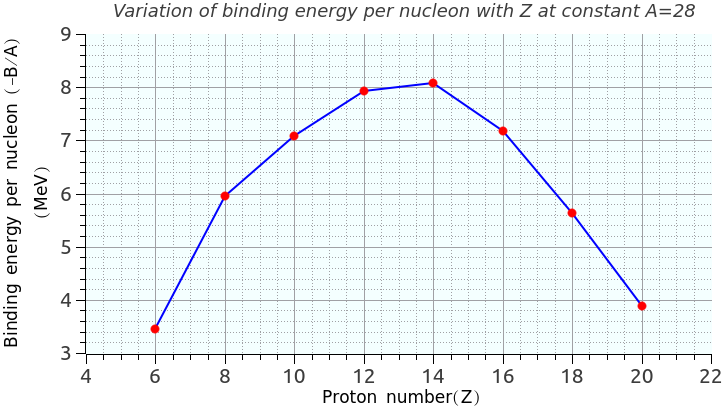
\includegraphics[width=0.50\textwidth,fbox]{image/BvsZ}
                        \caption{Binding energy per nucleus as a function of proton for a fixed mass number 28}
                        \label{BvsZ}
                    \end{figure}
                    \begin{wrapfigure}{r}{0.3\textwidth}
                        \centering
                        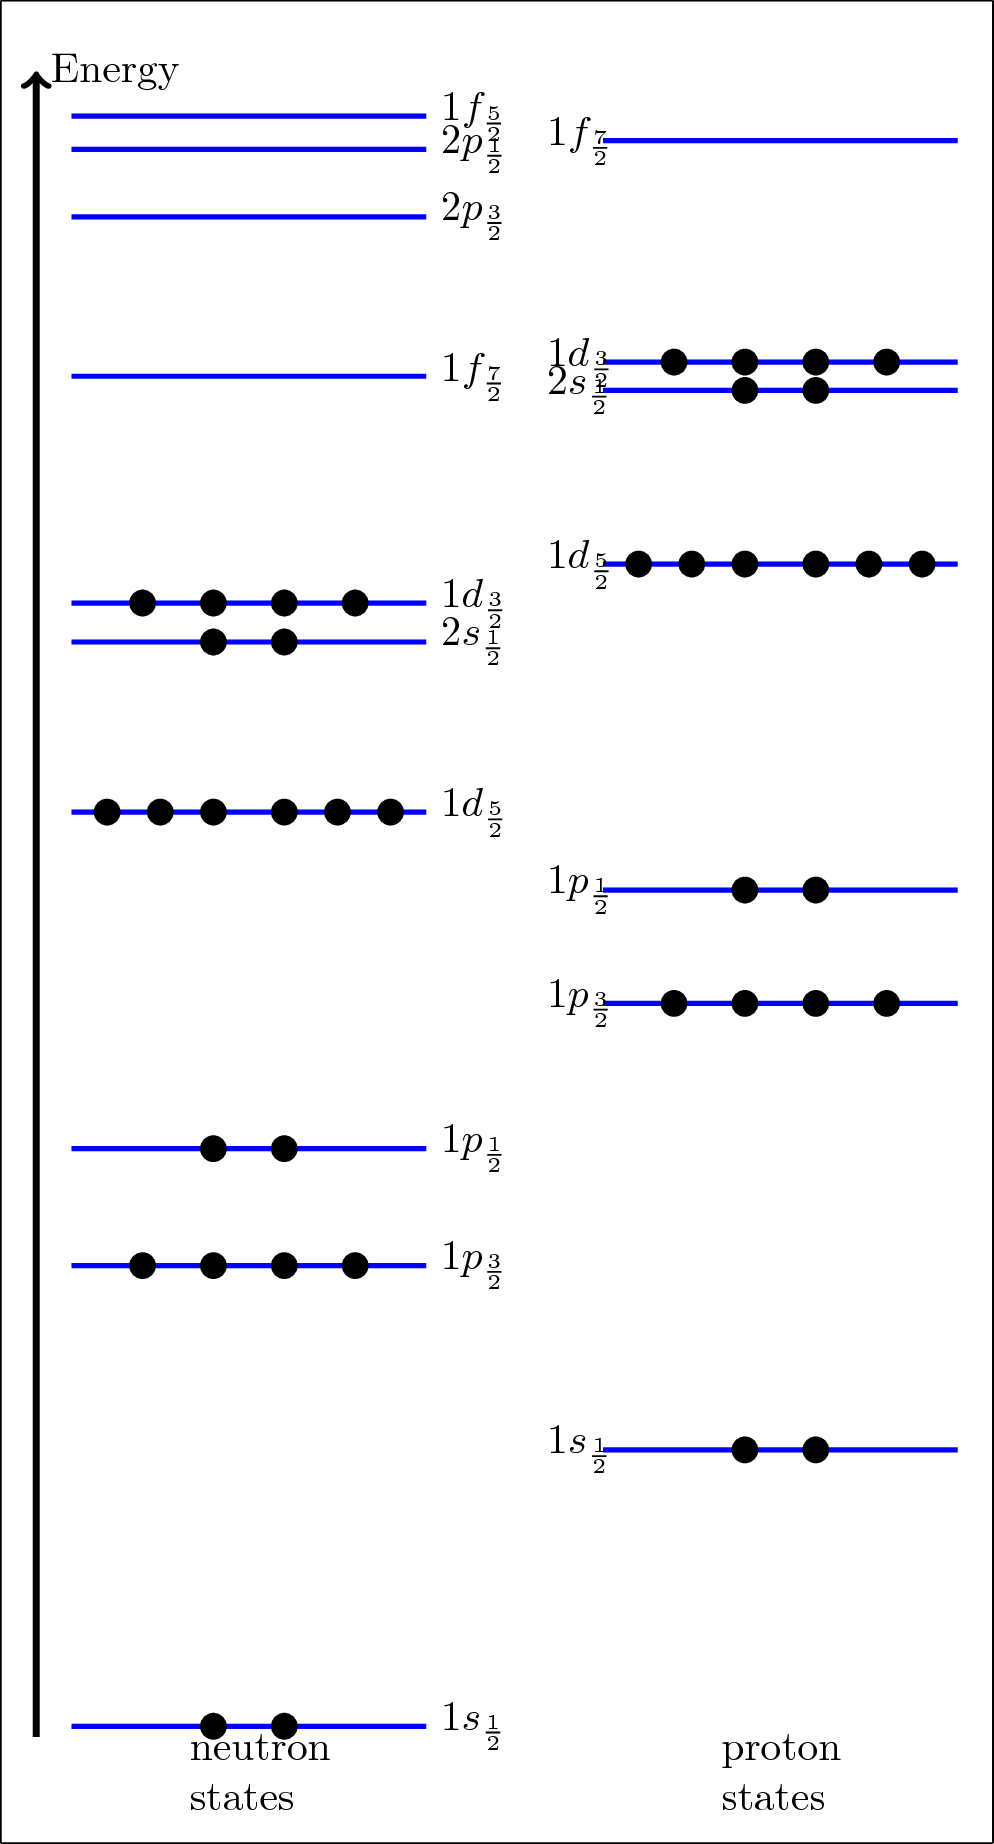
\includegraphics[width=0.3\textwidth]{image/levelCa40}
                        \caption{Energy level diagram for $Ca^{40}$; Single particle energy levels for proton(neutron) is shown on the left(right)}
                        \label{fig:Ca40level}
                    \end{wrapfigure}
                    Static Hartree-Fock method can be used to calculate many ground state properties of a nucleus. Energy levels of the ground state looks something like the figure \ref{fig:Ca40level}. Large energy gaps at magic numbers can be seen clearly. Notice that states having neutrons are lower in energy than the corresponding proton states. This is because the Coulomb repulsion between protons.\\
                    Also from the output of the code one can obtain the nuclear binding energy per nucleon ($-B/A$). An example of $-B/A$ changing with proton and neutron number is shown in figure \ref{BvsZ}. As can be seen for a given atomic mass equal no of proton and neutron is most stable i.e have highest binding energy.
                \subsubsection{Octupole vibration}
                    Octupole vibration as discussed in the section  \ref{Linear} using operator of the type 
                    \begin{equation}
                        \hat{Q_3} = \sqrt{\frac{7}{16\pi}}\sum_{i=1}^{A}\left\{2\hat{x}(i)^3 - 3\hat{x}(i)\left[\hat{y}(i)^2 + \hat{z}(i)^2\right]\right\}
                    \end{equation}
                    
                    
                    where i is the index over the nucleons. Only the $3^{-}$ excited states will contribute to the octupole vibration. So if we follow the theory in the section \ref{Linear}, we can extract the $q_{\nu} = \langle\nu|\hat{Q}_3|0\rangle$ as well as the energy of the $3^{-}$ states from the strength function.
                    A typical oscillation looks like \ref{oscillation}
                    Fourier transform of this will give the strength function. Strength function corresponding to the above oscillation is shown. For $Ca^{40}$ peaks are seen at energies near 4.5 MeV and 10 MeV. Both of these corresponds to different $3^{-}$ states. The most collective states having energy close to 4.5 MeV.
                    \begin{wrapfigure}{l}{0.30\textwidth}
                        \centering
                        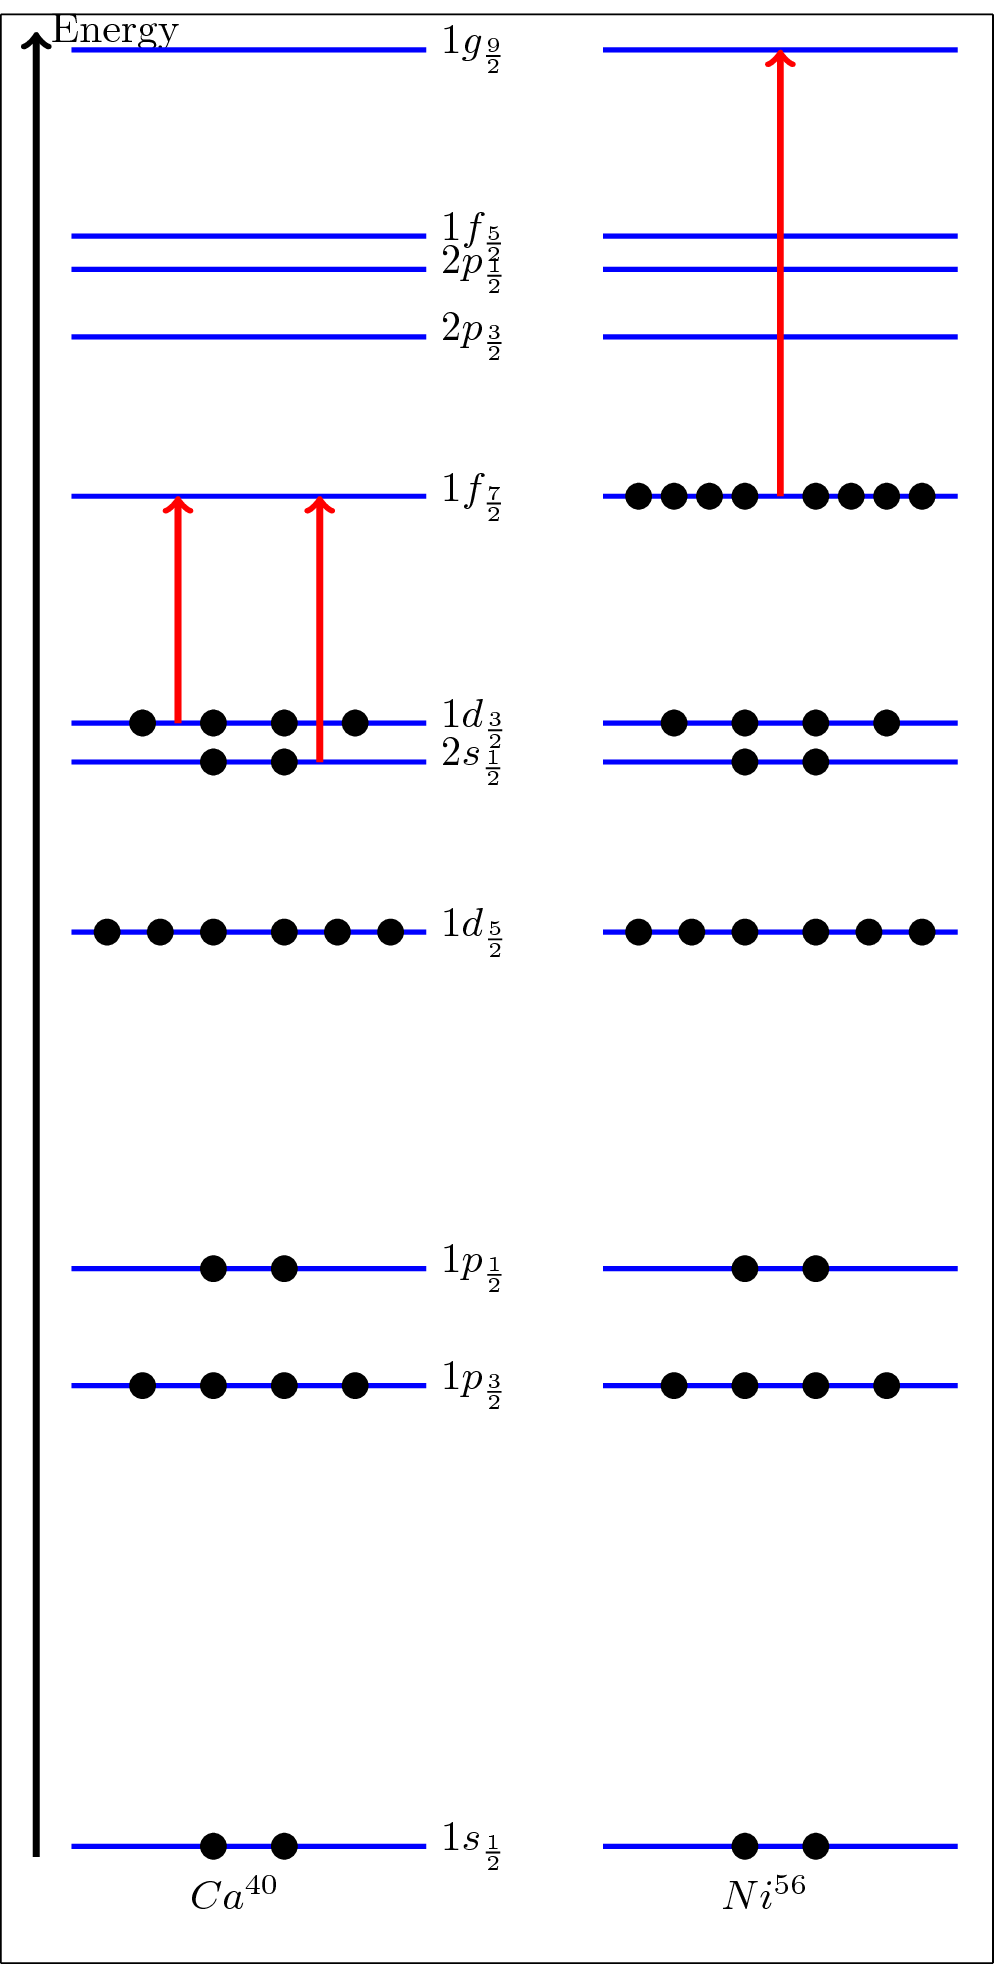
\includegraphics[width=0.30\textwidth]{image/levelCaNi}
                        \caption{Energy level diagram for $Ca^{40}$ (left) and $Ni^{56}$ (right); Transition energies: $Ca^{48}$ 6.4MeV, $Ni^{56}\approx$ 8MeV}
                        \label{fig:levelCaNi}
                    \end{wrapfigure} 
                    To understand the energies obtained in the strength function consider the energy level for $Ca^{40}$ and $Ni^{56}$ are shown (\ref{fig:levelCaNi}). The transitions which corresponds to  $3^{-}$ level and have energy close to the peak are shown with arrows. Here proton and neutron numbers are same in both cases so one should expect that same transitions are responsible for the collection of the strength function.\\
                    Note that the energy of the transitions are close to the energy of the $3^{-}$ states obtained from the strength function calculation but not exact matches. Reason being that in Quantum Mechanics one do not expect only one particle hole transition to contribute to the strength function.
                    Rather many 1p1h states contribute with different amplitudes (there is interference effect too!) hence slight change in the energies. Although the main contribution should come from the nearest particle hole transition energy. We will look into this in more detail taking $Ca^{48}$ as an example.\\
                    $Ca^{48}$ has $20$ protons and $28$ neutrons. So contribution from proton and neutrons are expected to be different. Note that protons are filled upto $1d_{\frac{3}{2}}$ while neutrons are filled upto $1f_{\frac{7}{2}}$. So it is expected that for neutrons strength function will be peaked at 10MeV as in $Ni^{56}$ while proton strength function will be peaked at 5MeV as in $Ca^{48}$. But the actual calculation shows the following picture \ref{fig:npstrength} which does not correspond to the anticipation made earlier. \\ 
                    As can be seen, even neutron strength function have a peak near energy 4MeV where no transition for the neutrons has similar energies which leads to a $3^{-}$ state! So it is entirely possible that higher energy transitions are contributing to this peak. Which ones? and How much? This question can not be answered using time-dependent Hartree-Fock calculation. We have to use different techniques. One such method is Random Phase Approximation(RPA). Results from RPA calculations are presented in the next subsection.
                    \begin{figure}
                        \centering
                        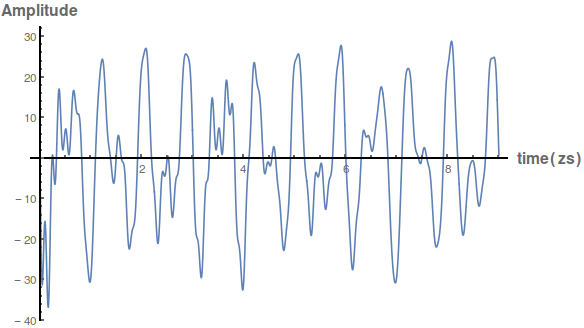
\includegraphics[width=0.8\textwidth,fbox]{image/Ca48moment}
                        \caption{Oscillation in octupole moment for a vibrating $Ca^{48}$ nucleus in linear regime}
                        \label{fig:Ca48moment}
                    \end{figure}
                    \begin{figure}[h]
                        \centering
                        \subfloat[Strength Function for $Ca^{40}$]{{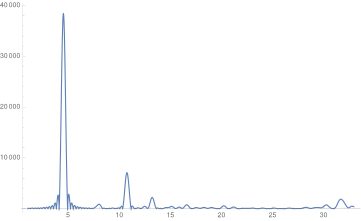
\includegraphics[width=0.45\textwidth,fbox]{image/Ca40strength}}}
                        \qquad
                        \subfloat[Strength Function for $Ni^{56}$]{{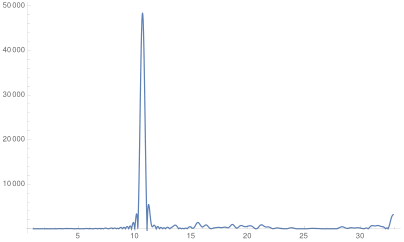
\includegraphics[width=0.45\textwidth,fbox]{image/Ni56strength}}}
                        \caption{Strength function of $Ca^{40}$ (left) and $Ni^{56}$ (right) shows peak corresponding to energies of the vibrational states in the respective nucleus; X-axis is in MeV}
                        \label{fig:strength}
                    \end{figure}
                    \begin{figure}[H]
                        \centering
                        \subfloat[Proton]{{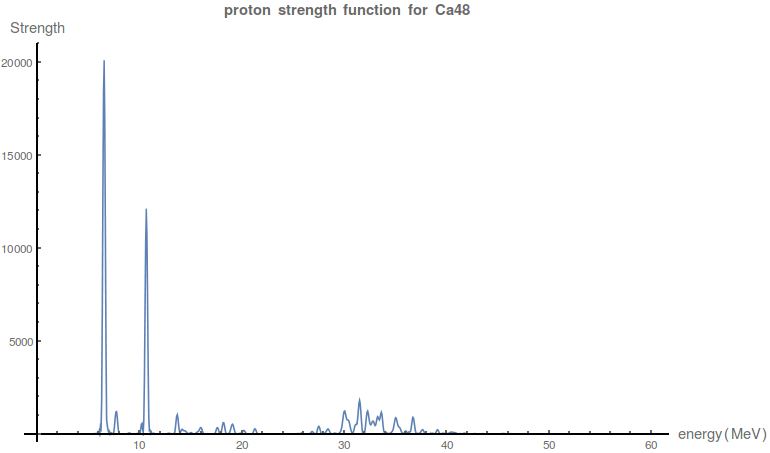
\includegraphics[width=0.45\textwidth,fbox]{image/Ca48strengthp}}}
                        \qquad
                        \subfloat[Neutron]{{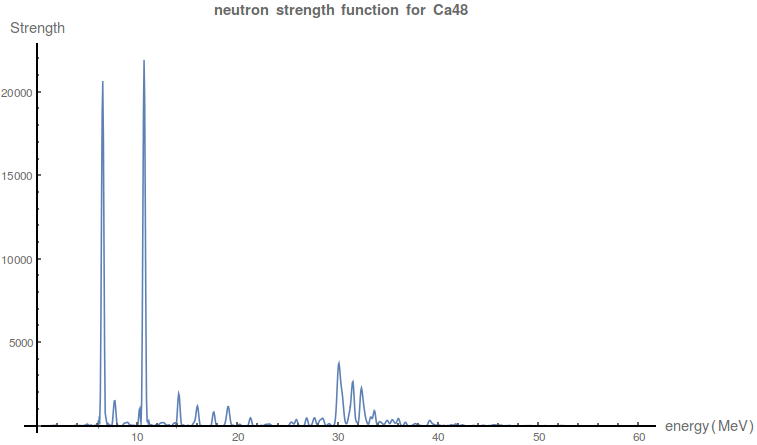
\includegraphics[width=0.45\textwidth,fbox]{image/Ca48strengthn}}}
                        \caption{Strength function for individual nucleons (proton and neutron) for $Ca^{48}$; Unexpected peak at 5 MeV for neutron strength function to be noted}
                        \label{fig:npstrength}
                    \end{figure}
            \subsection{Results from RPA}
                RPA is unique compared to TDHF as it is more accurate in computing excited state  \footnote{In Hartree-Fock one compute ground state using variational principle and use this approximate state to obtain the first excited state so error propagates with increasing energy states, while in RPA all states are calculated simultaneously}. Diagonalisation of the RPA matrix will give the energy levels ($3^{-}$) as its eigenvalues and from the eigenvector contribution from different particle-hole transition can be calculated. 
                Isoscalar and Isovector track the scalar and vector components of the transition respectively. In terms of proton and neutron's individual transition amplitude, they are given by
                \begin{subequations}
                    \begin{eqnarray}
                        IS = (p + n)^2 \\
                        IV = (p - n)^2
                    \end{eqnarray}
                \end{subequations}
                Only from the Isoscalar and Isovector data individual transition densities can not be extracted. But RPA code is able to give transition densities from different energy levels at different radius (from the centre of the nucleus). Compensating for an overall $r^2$ factor corresponding to the surface area, proton and neutron's indivudual transition densities can be obtained. Calculations for $Ca^{48}$ is shown below.
                \begin{figure}[h]
                    \centering
                        \subfloat[Isoscalar]{{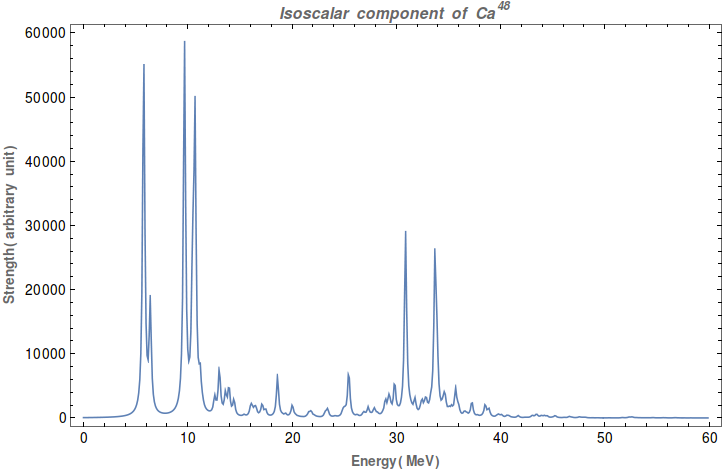
\includegraphics[width=0.45\textwidth,fbox]{image/Ca48isoscalar}}}
                        \qquad
                        \subfloat[Isovector]{{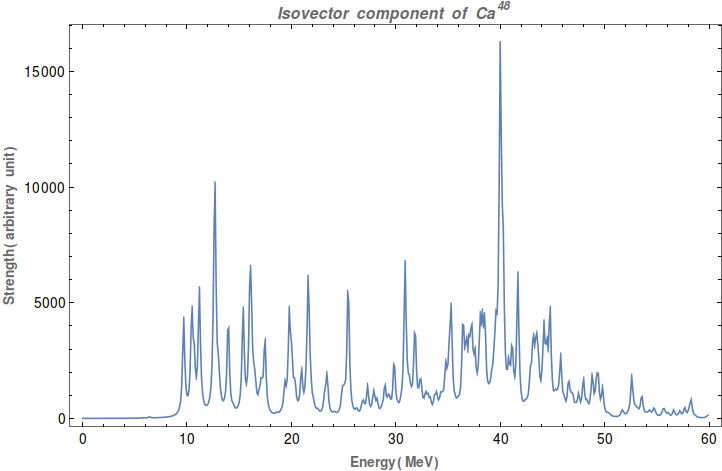
\includegraphics[width=0.45\textwidth,fbox]{image/Ca48isovector}}}
                        \caption{Isoscalar and Isovector components of the $3^-$ transition in $Ca^{48}$.}
                        \label{fig:rpaisiv}
                \end{figure}
                \begin{figure}[h]
                    \centering
                       
                        \subfloat[Proton]{{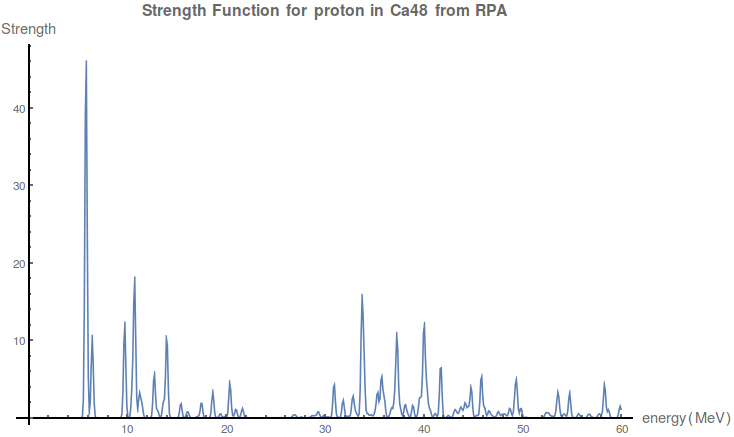
\includegraphics[width=0.45\textwidth,fbox]{image/Ca48strengthprpa}}}
                        \qquad
                        \subfloat[Neutron]{{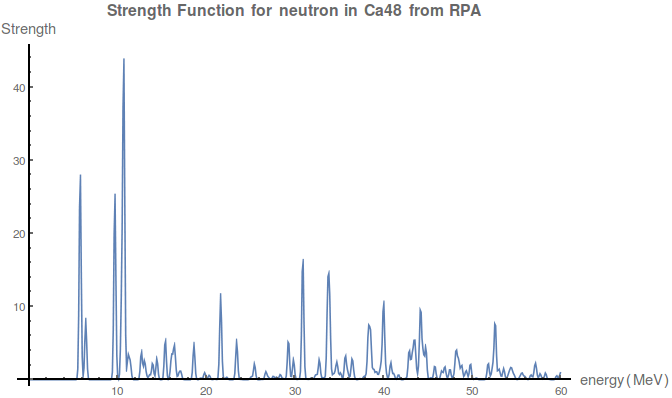
\includegraphics[width=0.45\textwidth,fbox]{image/Ca48strengthnrpa}}}
                        \caption{Neutron(right) and Proton(left) transition strengths as a function of the energy for $Ca^{48}$.}
                        \label{fig:rpapn}
                \end{figure}
                
                Note that even in the RPA calculation there is a peak at 5 MeV in neutron strength function, this supports our previous calculation using TDHF. But still, it is left to understand the origin of this peak. \\
                To understand the composition of the first RPA state first we calculate the eigenvectors of the RPA matrix which gives the X and Y values(see \ref{eqn:RPAeqn}). For this specific calculation of $Ca^{48}$, Y values are small compared to the X values. So we can neglect the Y's and adopt the Tamm-Dancoff Approximation. Then the values X have special meaning. $|X_{mi}^{\nu}|^2$ gives the probability of obtaining the $\mathbf{a}^{\dagger}\mathbf{a}|RPA\rangle$ in the state $|\nu\rangle$. But again $\mathbf{a}^{\dagger}_{m}\mathbf{a}_{i}|RPA\rangle$ is not exactly the 1p1h state we are looking for. But upto an approximation this probability is equal to that of 1p1h state $\mathbf{a}^{\dagger}_{m}\mathbf{a}_{i}|HF\rangle$. Then X's will denote the contribution of 1p1h states to any RPA state. Values of X are plotted below for the first excited state.
                \begin{figure}[H]
                \centering
                    \subfloat[Contributions from 1p1h states]{{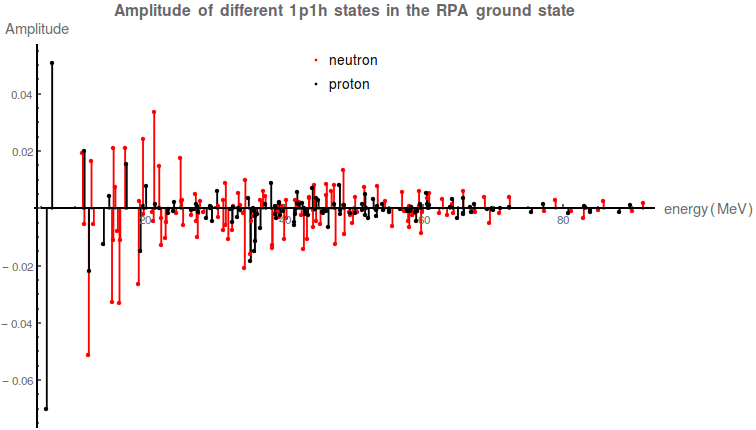
\includegraphics[width=0.70\textwidth,fbox]{image/Ca48contribution1p1h}}}
                    \subfloat[]{{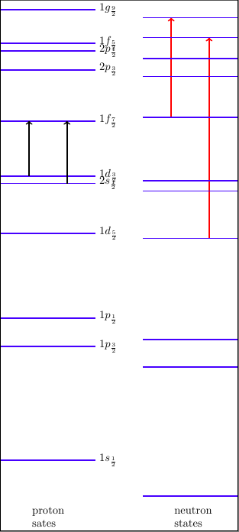
\includegraphics[width=0.18\textwidth,fbox]{image/Ca48rpalevel}}}
                    \caption{(a) Contribution from each single particle hole transition(protons in black and neutrons in red) to the RPA ground state. (b) Energy levels of protons (left) and neutrons(right) in $Ca^{48}$.}
                \end{figure}

                From the above figure as can be seen there are a significant contribution from the higher energy transition as well. Low energy transitions which are anticipated to be contributing most are contributing only 5-10 \% . Though in the above calculation we made two assumptions one neglecting Y's and two approximating RPA ground state with Hartree-Fock ground state. The first one is easy to verify against by just checking the Y/X values. the second one is little bit more  involved. One has to construct the RPA ground state. Construction details can be found in the section 8.4.6 of reference \ref{ref:nuclearmany} or 11.3.2 of reference \ref{ref:nucleonstonucleus}.
                
        \begin{appendices}\label{appendices}
            \section{code TDHF}
            \section{code RPA}
            The code for RPA calculation is taken from \ref{ref:rpacode}. A few changes has been made to obtain the 1p1h contributions (X values).
            The code first uses Hartree-Fock method to compute the mean field. Then uses this information to carry out RPA calculations. Given the Skyrme-force parameter, mesh sizes etc. as input it gives the following outputs (relevant for this case). 
            \begin{itemize}
                \item Isoscalar and Isovector 
                \item Proton neutron transition densities at different radius for each RPA states.
                \item The main output file containing information about the possible 1p1h states, RPA states and their energies etc.
            \end{itemize} 
            As said earlier knowledge of just Isoscalar and Isovector is not enough to obtain proton neutron transition densities. But we have proton neutron transition densities at different radii. So we can add all the transition densities with a factor of $r^2$ which compensate for the surface area. Also one can print the matrix A and B and then construct the RPA matrix oneself. Diagonalisation of that matrix will give X and Y values as well as the RPA energies.
        \end{appendices}
        \section*{References}
        \begin{enumerate}
            \item Suhonen J. (2007) \textbf{From Nucleons to Nucleus}: Concepts of Microscopic Nuclear Theory : Springer. DOI : 10.1007/978-3-540-48861-3.\label{ref:nucleonstonucleus}
            \item Ring P., Schuck P. (1980) \textbf{The Nuclear Many-Body Problem}: Springer.\label{ref:nuclearmany}
            \item Self-consistent RPA calculations with Skyrme-type interactions: The skyrme-rpa program \label{ref:rpacode}
            %/\\item Taqi A. H.,Ali M. S. (2017) \textbf{Self-consistent Hartree–Fock RPA calculations in $Pb^{208}$}
            
        \end{enumerate}
    \end{document}